\documentclass[a4paper,DIV=12,english]{scrartcl}
\usepackage[utf8]{inputenc}
\usepackage{fancyhdr}
\usepackage{bookmark}
\usepackage{graphicx}
\usepackage{hyperref}
\usepackage{xurl}
\usepackage[sorting=none, style=numeric-comp]{biblatex}
\addbibresource{ref.bib}
\usepackage{csquotes}
\usepackage[dvipsnames]{xcolor}
\usepackage[num]{isodate}
\usepackage{amsthm}
\usepackage{amssymb}
\usepackage{bbm}
\usepackage{amsmath}
\usepackage{tikz}
%\usepackage{pgfplots}
    %\usepgfplotslibrary{fillbetween}
\usepackage{svg}
\usepackage{braket}
\usepackage{caption}
\usepackage{subcaption}
\usepackage{placeins}
%\setlength\parindent{0pt}
\usepackage{wrapfig}
\usepackage{float}

% Fakesection
\newcommand{\fakesection}[1]{%
    \par\refstepcounter{section}                                        % Increase section counter
    \sectionmark{#1}                                                    % Add section mark (header)
    \addcontentsline{toc}{section}{\protect\numberline{\thesection}#1}  % Add section to ToC
    % Add more content here, if needed.
} 

\renewcommand{\footrulewidth}{0.5pt}
\pagestyle{fancy}
\fancyhf{}
\fancyhead[L]{\leftmark}
\fancyhead[R]{}

\fancyfoot[C]{Computational Physics: Band Structure of Lithium using Augmented Plane Waves}
\fancyfoot[R]{\thepage}

\title{Computational Physics: Calculating the Band Structure of Lithium using Augmented Plane Waves}
\author{Stockholm University, Spring Term 2024 \\Max Maschke}
\date{May 14 2024}


\begin{document}
\maketitle


\tableofcontents
\newpage


\newpage
\section{Introduction}\cite{github}

\section{Electronic States in Periodic Potentials}
Solid state systems such as metallic crystals contain on the order of $10^{23}$ electrons. Their collective behaviour is what determines the bulk properties of the material. A major reason why these properties are at all computationally tractable is symmetry. A crystal (Bravais) lattice in 3D is defined by the fact that there is a set of elementary translation vectors $\{\textbf{a}_1, \textbf{a}_2, \textbf{a}_3\}$ from which every point $\textbf{R}$ or the lattice can be constructed using an integer linear combination:
\begin{equation}
    \textbf{R} = l\textbf{a}_1 + m\textbf{a}_2 + n\textbf{a}_3, \quad l,m,n\in\mathbb{Z}
\end{equation}
This discrete translational symmetry has major implications. Assuming from now on a one-particle picture in which we ignore any interactions of valence and conduction electrons, the electrons feel a potential caused by the ions and core electrons localised at the lattice sites. Because these lattice sites are periodic, the potential is also periodic, i.e.
\begin{equation}
    V(\textbf{r} + \textbf{R}) = V(\textbf{r}).
\end{equation}

\subsection{The Reciprocal Lattice}
The reciprocal lattice is the set of wave vectors $\{\textbf{K}\}$ whose associated plane waves $\text{e}^{i\textbf{k}\textbf{r}}$ are compatible with the periodicity of the real space or direct lattice defined by its elementary translations. That is, it must obey
\begin{equation}
    \textbf{a}_i \cdot \textbf{b}_j = 2\pi \delta_{ij}
\end{equation}
It is obtained via a Fourier transform of the direct lattice and has its own set of elementary lattice vectors
\begin{equation}
    \textbf{b}_1 = \frac{2\pi}{V} \textbf{a}_2 \times \textbf{a}_3 \quad \text{and cyclic.}
\end{equation}
Here, $V=\textbf{a}_1 \cdot (\textbf{a}_2 \times \textbf{a}_3)$ is the volume of the unit cell of the direct lattice~\cite{theoFestkörper}.

\subsection{Bloch's Theorem}
Due to the periodicity of the potential, it has a Fourier representation
\begin{equation}
    V(\textbf{r}) = \sum_\textbf{K} V_\textbf{K} \text{e}^{i\textbf{K}\textbf{r}} 
\end{equation}
where the sum runs over the reciprocal lattice.

Similarly, but distinctly, we can represent a given single particle wave function $\psi$ as 
\begin{equation}
    \psi(\textbf{r}) = \sum_\textbf{q} c_\textbf{q} \text{e}^{i\textbf{q}\textbf{r}} 
\end{equation}
where the sum runs over all wave vectors compatible with the boundary conditions. For infinite system, this becomes an integral over all of $\mathbb{R}^3$.

Plugging both into the single particle Schrödinger equation, one can show without great difficulty~\cite{Thijssen2007cp} that with $\textbf{k}=\textbf{q} + \textbf{K}$ the eigenstates have the form 
\begin{equation}
    \psi_\textbf{k}(\textbf{r}) = \text{e}^{i\textbf{k}\textbf{r}} u_\textbf{k}(\textbf{r})
\end{equation}
where $u$ is a function that shares the periodicity of the lattice. This is known as Bloch's theorem. Its power lies in the fact that it is sufficient to limit ones' analysis to the momenta inside a unit cell of the reciprocal lattice to describe the states of the whole direct lattice. Usually, one chooses the first Wigner-Seitz cell of the reciprocal cell for this purpose, which is also known as the first Brillouin zone.

\subsection{Tight Binding vs Quasi-Free Electrons}
The question of what the dispersion $E(\textbf{k})$\footnote{$E(\textbf{k})$ is usually not a unique function, to uniquely describe an electronic state, the entire tuple ($E$, \textbf{k}) (and possibly $\sigma$) must be specified.} of the lattice electrons looks like is at the core of band structure analysis and its answer can give fundamental insights into a material's properties, such as whether it conducts electric currents.

There are two very simple approaches to this question that have since been built upon, which make qualitatively very different assumptions.

A tight binding approach assumes the valence electrons are localised at the lattice sites\footnote{It is not necessarily obvious what these localised states should look like. The Wannier basis is a popular choice.} but can transition between them with some amplitude $t$. For a simple 1D chain with lattice constant $a$, such a model might read 
\begin{equation}
    \mathcal{H} = \sum_{i, \sigma} t \left( c^\dagger_{i,\sigma} c_{i+1,\sigma} + c^\dagger_{i+1,\sigma} c_{i,\sigma}\right).
\end{equation}
This can be directly solved via a Fourier transform and the dispersion is~\cite{theoFestkörper}
\begin{equation}
    \varepsilon_k = -2t\cos(ka) + \text{const}.
\end{equation}
Cosine-shaped bands are typical for tight binding calculations.

The other approach is to start from free electrons, which have a quadratic dispersion $E\sim k^2$ and whose wave functions are plane waves, and apply perturbation theory. The advantage of this approach is that it is able to produce gaps between energy bands.

However, both approaches are incredibly basic and only rarely accurately describe the true band structure of real crystals. They are however instructive as starting points from which to understand more sophisticated methods.


\section{Augmented Plane Waves}
We have recalled that assembling electronic states from neither plane waves nor atomic wave functions is incredibly successful on its own. One might then reasonably ask whether any improvements are to be gained by combining both ideas somehow. In a seminal paper~\cite{SLATER196435}, Slater proposed just this in an approach which is now known as augmented plane waves (APW). The idea is to compose the state from the atomic functions close to the ions and from plane waves further out.

\subsection{The Muffin Tin Approximation and Muffin Tin Orbitals}
By choosing a radius $R$ around the ions in which we assume the electrons to be comparatively strongly bound and thus described by a superposition of atomic states, we're performing what's known as the muffin tin approximation. These atomic states are not eigenstates but are solutions at a prescribed energy $E$. For systems with one valence electron, they may be obtained by first finding a reasonable single particle potential and then shooting the solutions from $r=0$ to $R$ using an iterative solver such as the ever-popular RK4.

The potential $V(r)$ is in our case obtained using the DFT code previously produced for this course, which was based on the local density approximation.

We then iterate the equation for the radial function $P_{l,E}(r)$ for a given energy $E$ and $l$
\begin{equation}
    \partial_r^2 P_{l,E}(r) = \left(\frac{l(l+1)}{r^2} + 2V(r) - 2E\right)P_{l,E}(r)
\end{equation}
using the initial conditions
\begin{equation}
    P_{l,E}(r) = 0, \quad \partial_r P_{l,E}(r)|_{r=0} = r^l.
\end{equation}
Note that $P_{l,E}(r)/r = R_{l,E}(r)$ is the radial wave function.

\subsection{Constructing the Augmented Basis}
The $R_{l,E}$ depend on the choice of $E=k^2/2$ for a given plane wave $\text{e}^{i\textbf{k}\textbf{r}}$, while the latter also depends on the orientation of $\textbf{k}$. Matching them at the muffin tin boundaries is thus slightly non-trivial and results in a discontinuous derivative with functions of the form~\cite{Thijssen2007cp} 
\begin{equation}
    \psi^{\text{APW}}_\textbf{k} (\textbf{r}) = 4\pi \sum_{lm}i^l j_l(kR)\frac{R_{l,k^2/2}(r)}{R_{l,k^2/2}(R)} Y^{l*}_m (\theta_k, \varphi_k)
    Y^{l}_m (\theta_r, \varphi_r)
\end{equation}
where $j_l$ are the spherical Bessel functions and the $Y^l_m$ the spherical harmonics. The sum does in principle run over all allowed values of $l$ and $m$ but is in practice truncated to some $l_\text{max}$ which we chose as 6.

\subsection{Solving for the Electronic States}
We want to find Bloch states for the valence electrons of the form 
\begin{equation}
    \psi_\textbf{k}(\textbf{r}) = \sum_\textbf{K} c_\textbf{K} \psi^{\text{APW}}_{\textbf{k} + \textbf{K}}(\textbf{r}),
\end{equation}
where the sum over all reciprocal lattice vectors is in practice truncated beyond some cut-off $K_\text{max} = |\textbf{K}_\text{max}|$.
The coefficients $\textbf{c}$ minimise the energy mismatch inside and outside the muffin tins. Finding them is rather complicated as they are given by the solutions of a matrix equation 
\begin{equation}\label{eq:evalprob}
    (H_E - EI)\textbf{c} = 0
\end{equation}
where the matrix $H_E$ depends on energy, which prevents us from using the usual tools of linear algebra for solving eigenvalue problems. The matrix elements are given by~\cite{Thijssen2007cp}
\begin{align}
    H_{ij} &= \braket{\textbf{k}+\textbf{K}_i|H_E|\textbf{k}+\textbf{K}_j} = -E\,A_{ij} + B_{ij} + \sum_l C_{ijl} \frac{R'_{l, E}(R)}{R_{l, E}(R)} \\
    A_{ij} &= -\frac{4\pi R^2}{V} \frac{j_1\left( \left|\textbf{K}_i - \textbf{K}_j\right|\cdot R \right)}{\left|\textbf{K}_i - \textbf{K}_j\right|} + \delta_{ij} \\
    B_{ij} &= \frac{1}{2}A_{ij}\, \left(\textbf{k}+\textbf{K}_i\right) \cdot \left(\textbf{k}+\textbf{K}_j\right) \\
    C_{ijl} &= (2l+1)\frac{2\pi R^2}{V} P_l\left(\frac{\left(\textbf{k}+\textbf{K}_i\right) \cdot \left(\textbf{k}+\textbf{K}_j\right)}{\left|\textbf{k}+\textbf{K}_i\right| \left|\textbf{k}+\textbf{K}_j\right|}\right) j_l(\left|\textbf{k}+\textbf{K}_i\right|R) j_l(\left|\textbf{k}+\textbf{K}_j\right|R).
\end{align}
Note that here, $P_l$ denotes the Legendre polynomials and not a radial function.

Given the unfavourable structure of~\eqref{eq:evalprob}, one is forced to find the generalised eigenvalues $E$ which give the dispersion by scanning a dense discrete interval of energies and calculating the determinant $\det\left(H_E - EI\right)$.

\section{Solid State Lithium}
\begin{figure}
    \centering 
    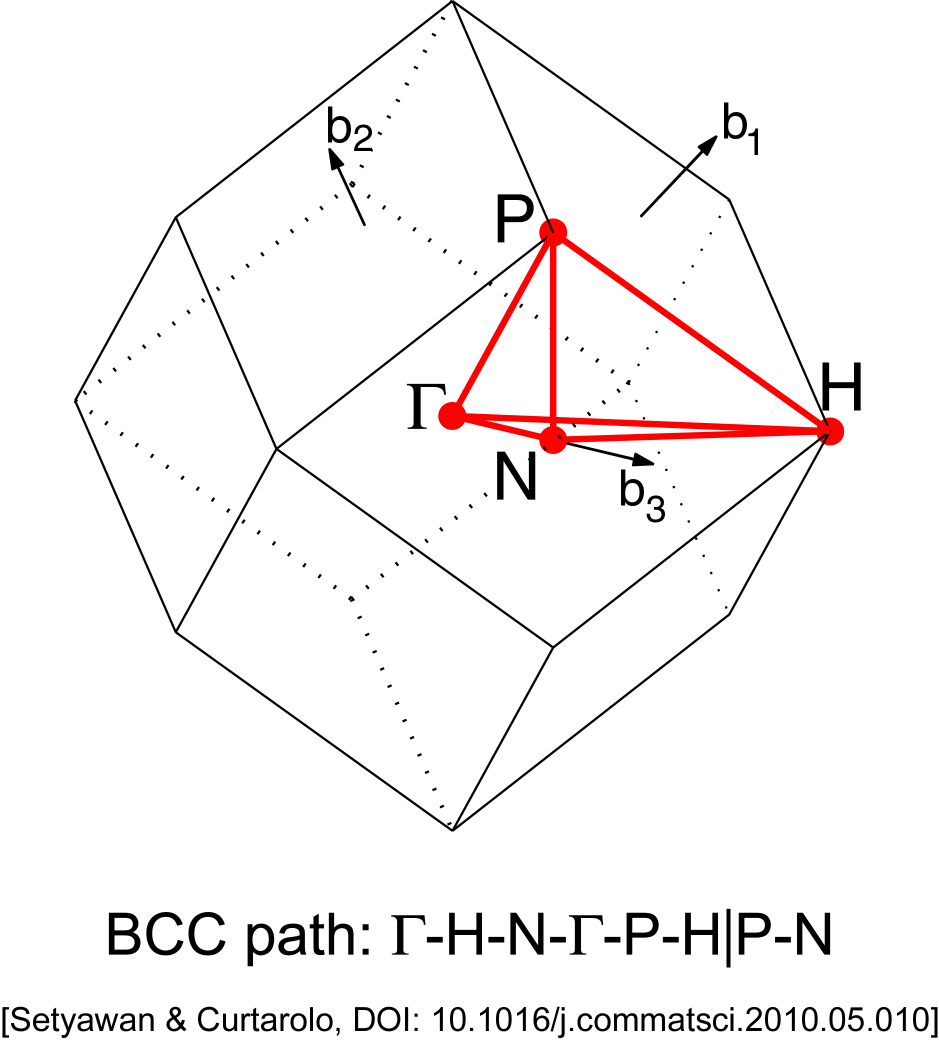
\includegraphics[width=0.55\textwidth]{./fig/bcc_bz.png}
    \caption{Brillouin zone for a BCC lattice. The indicated path follows high symmetry directions of the BZ. Image credit indicated.}
    \label{fig:bcc_bz}
\end{figure}
Lithium is the third element of the periodic table, consisting of a triply charged nucleus and three electrons. As an alkaline metal, it is soft and highly reactive. Nevertheless, it is crystalline in the bulk, growing body centric cubic (BCC) lattices with lattice constant $a=350.0\,\text{pm}=6.632\,a_0$~\cite{wikiLithium}. The Brillouin zone (BZ) of the BCC lattice is shown in figure~\ref{fig:bcc_bz}.

The electronic structure of Lithium atoms is $1s^22s^1$ in the orbital picture. In this analysis, we only consider the valence electron to be responsible for Lithiums band structure.

\FloatBarrier
\section{Numerical Implementation}

\FloatBarrier
\section{Results}

\FloatBarrier
\section{Conclusion}


\FloatBarrier
\newpage
\fakesection{References}
\printbibliography


\end{document}
